%%%%%%%%%%%%%%%%%%%%%%%%%%%%%%%%%%%%%%%%%%%%%%%%%%%%%%%%%%%%%%%%%%%%%%%%%%%%%%%%%%%%%%%%%%
%%
%% Description:		This is an example presentation using the beamerthemedhbw
%%
%%					The beamerthemedhbw is based on jacksbeamertheme
%%					(https://github.com/JacknJo/jacksbeamertheme)
%%
%% Author:			Hannes Bartle																				
%% 					DHBW Ravensburg Campus Friedrichshafen		
%%					September 2016	
%% 
%% The beamerthemedhbw is free software: you can redistribute it and/or modify
%% it under the terms of the GNU General Public License as published by
%% the Free Software Foundation, either version 3 of the License, or
%% (at your option) any later version.
%% 
%% The beamerthemedhbw is distributed in the hope that it will be useful,
%% but WITHOUT ANY WARRANTY; without even the implied warranty of
%% MERCHANTABILITY or FITNESS FOR A PARTICULAR PURPOSE.  See the
%% GNU General Public License for more details.
%% 
%% You should have received a copy of the GNU General Public License
%% along with the beamerthemedhbw.  If not, see <http://www.gnu.org/licenses/>.
%% 
%% 
%%%%%%%%%%%%%%%%%%%%%%%%%%%%%%%%%%%%%%%%%%%%%%%%%%%%%%%%%%%%%%%%%%%%%%%%%%%%%%%%%%%%%%%%%%


\documentclass[	12pt, 				
				t,					
				aspectratio=169,
				%handout-PLACEHOLDER
				]{beamer}

\usepackage{dhbwstyle}

\title{Algorithmen}

\begin{document}
	
	\begin{frame}[noframenumbering]
		\titlepage
	\end{frame}


	\begin{frame}{Outline}
		\tableofcontents
	\end{frame}

    \outlineFrame{Allgemeines}

    \begin{frame}{Multithreading}{Allgemeines (Vgl. \cite{ullenboom2018java} S. 948)}
    \begin{itemize}
        \item Moderne Betriebssysteme unterstützen \textit{Multitasking}
        \item Bedeutet: Mehrere Programme können gleichzeitig laufen
        \item Man spricht in der Regel von \textit{Nebenläufigkeit}
        \item Wie diese erreicht wird steuert das Betriebssystem (und ggf. Hardware)
        \item Auf Mehrkernprozessoren können "`echt parallel"' arbeiten
        \item Auf Einkernsystemen wird eine Parallelität "`simulisert"' (\textit{Quasiparallelität})
    \end{itemize}
\end{frame}

\begin{frame}{Multithreading}{Technische Umsetzung (Vgl. \cite{ullenboom2018java} S. 948)}
    \begin{itemize}
        \item Jeder Prozessorkern kann (in der Regel) zu einem Zeitpunkt einen Prozess bearbeiten
        \item In der Regel gibt es deutlich mehr laufende Prozesse als Kerne
        \item Lösung: Aktiver Prozess wird auf den Kernen hochfrequent (im Millisekundenbereich) umgeschalten
        \item Umschaltung erfolgt durch den \textit{Scheduler}
        \item Zur Umschaltung der Prozesse gibt es diverse Strategien mit diversen Parametern:
        \begin{itemize}
            \item Priorität
            \item Bearbeitungsdauer
            \item "`Fail-Count"' -- Wie oft wurde der Prozess schon versucht zu bearbeiten
        \end{itemize}
    \end{itemize}
\end{frame}

\begin{frame}{Prozesse}{Grundlegende Eigenschaften (Vgl. \cite{ullenboom2018java} S. 948)}
    \begin{itemize}
        \item Jeder Prozess besteht im Grunde aus:
        \begin{itemize}
            \item Dem auszuführenden Programmcode
            \item Den dazugehörigen Daten
            \item Einem \textit{eigenen} (isolierten) Speicherbereich
            \item Ggf. Verwendete Ressourcen wie Dateien oder Laufwerke
        \end{itemize}
        \item Durch die Trennung des Speicherbereichs können Prozesse nicht auf die Daten anderer Prozesse zugreifen!
        \item Ist doch ein Datenaustausch zwischen Prozessen erforderlich, ist ein spezielle \textit{Shared Memory} Bereich notwendig
        \item Prozesse können aus mehreren parallelen Threads bestehen $\rightarrow$ Diese können die gleichen Ressourcen nutzen
    \end{itemize}
\end{frame}

\begin{frame}{Nebenläufigkeit}{Geschwindigkeitsgewinn (Vgl. \cite{ullenboom2018java} S. 949ff)}
    \begin{itemize}
        \item Nebenläufigkeit führt in der Regel zu Geschwindigkeitsgewinn
        \item In Mehrkernsystemen sowieso...
        \item ...aber auch in Einkernsystemen
        \item Beispiel: Software zur Erstellung von Datenbank-Reports:
        \begin{itemize}
            \item Baue ein Fenster auf
            \item Öffnen der Datenbank vom Server, lesen der Datensätze
            \item Analyse der Daten, Visualisierung des Fortschritts
            \item Datei öffnen, Analyseergebnisse in Datei schreiben
        \end{itemize}
    \end{itemize}
\end{frame}

\begin{frame}{Nebenläufigkeit}{Beispiel für Geschwindigkeitsgewinn (Vgl. \cite{ullenboom2018java} S. 949ff)}
    \begin{itemize}
        \item Betrachten wir einmal die parallelisierbaren Abschnitte:
        \begin{itemize}
            \item Öffnen von Fenster und Datenbank können parallel geschehen
            \item Lesen neuer Datensätze und Analyse alter Datensätze kann parallel erfolgen
            \item Analyse neuer Datensätze und schreiben von alten analysierten Daten kann gleichzeitig abgearbeitet werden
        \end{itemize}
        \item Hier auch auf einem Einprozessorsystem großer Leistungsgewinn
        \item Da die parallelen Prozesse verschiedene \textit{Ressourcen} belasten
    \end{itemize}
\end{frame}

\begin{frame}{Nebenläufigkeit}{Beispiel für Geschwindigkeitsgewinn (Vgl. \cite{ullenboom2018java} S. 949ff)}
    \begin{itemize}
        \item Während auf das Fertigstellen einer Ressource gewartet wird, können Aufgaben bearbeitet werden die andere Ressourcen benötigen:
        \begin{itemize}
            \item Während der Prozessor ausgelastet ist die GUI zu erstellen kann eine Datei auf der Festplatte geöffnet werden $\rightarrow$ Dateioperationen benötigen wenig Prozessorleistung, eher durch Festplattengeschwindigkeit begrenzt
            \item Während Daten z.B. aus einer Datenbank abgerufen werden wird hauptsächlich die Netzwerkressource belastet $\rightarrow$ Prozessorleistung kann ggf. anders genutzt werden
            \item Parallel zu einer Prozessorlastigen Analyse können bereits analysierte Daten in eine Datei geschrieben werden
        \end{itemize}
        \item Kurz gesagt: Wir nutzen "`Wartezeiten"' von langsamen Operationen zu unserem Vorteil
    \end{itemize}
\end{frame}

\begin{frame}{Nebenläufigkeit}{Fazit (Siehe \cite{ullenboom2018java} S. 951)}
    \begin{itemize}
        \item Nebenläufigkeit muss gut geplant werden
        \item Insbesondere für Einkernsysteme
        \item Geschwindigkeitsgewinn nur vorhanden, wenn die parallelen Aktivitäten unterschiedliche Ressourcen nutzen
        \item Durch Nebenläufigkeit entsteht auch ggf. zusätzlicher Overhead für Synchronisation
        \item Zum Beispiel, wenn auf ein Teilergebnis gewartet werden muss
        \item Hier muss insbesondere auf konkurrierende Zugriffe und gegenseitige Wartebedingungen geachtet werden, um \textit{Deadlocks} zu vermeiden
    \end{itemize}
\end{frame}



    \outlineFrame{Beschreibung}
    \outlineSubframe{Formale Eigenschaften}

\begin{frame}{Eigenschaften von Algorithmen}{Grundlegendes}
    \begin{itemize}[<+->]
        \item \textbf{Finitheit} - Ein Algorithmus lässt sich in endlch vielen Schritten eindeutig beschreiben
        \item \textbf{Ausführbarkeit} - Jeder Einzelschritt muss tatsächlich ausführbar sein
        \item \textbf{Platzkomplexität} - Ein Algorithmus benötigt zu jedem Zeitpunkt nur endlich viel Speicherplatz
        \item \textbf{Terminierung} - Der Algorithmus benötigt eine endliche Anzahl von Schritten zur Ausführung
        \item \textbf{Determiniertheit} - Der Algorithmus muss bei gleichen Rahmenbedingungen das gleiche Ergebnis liefern
        \item \textbf{Determinismus} - Der nächste Schritt des Algorithmus ist zu jedem Zeitpunkt genau definiert
    \end{itemize}
\end{frame}

\begin{frame}{Effizienz von Algorithmen}{}
    \begin{itemize}
        \item Ergibt sich indirekt aus den Grundlegenden Eigenschaften
        \item Effizienz lässt sich über verschiedene Größen beschreiben:
        \begin{itemize}
            \item Speicherverbrauch
            \item Zeitverbrauch
        \end{itemize}
        \item Die sind jedoch oft Implementierungs- und Rechnerabhägig
        \item Deshalb wird mit formalisierten Modellen gearbeitet
        \item ...Mehr dazu im Kapitel "`Analyse"'
    \end{itemize}
    
    Vgl. \cite{ottmann2017}, S. 2f
\end{frame}

\outlineSubframe{Darstellungsformen}

\begin{frame}[fragile]{Ein kleines Beispiel}{Warum wir das überhaupt brauchen (Algorithmus siehe \cite{wiki:qrsqrt})}
\lstset{style=cpp}
\begin{onlyenv}<1|handout:0>
\begin{lstlisting}
float Q_rsqrt( float number ){
  long i;
  float x2, y;
  const float threehalfs = 1.5F;

  x2 = number * 0.5F;
  y  = number;
  i  = * ( long * ) &y;                       
  i  = 0x5f3759df - ( i >> 1 );                
  y  = * ( float * ) &i;
  y  = y * ( threehalfs - ( x2 * y * y ) );   
//y  = y * ( threehalfs - ( x2 * y * y ) );   
  return y;
}
\end{lstlisting}
\end{onlyenv}
\begin{onlyenv}<2>
\begin{lstlisting}
float Q_rsqrt( float number ) {
  long i;
  float x2, y;
  const float threehalfs = 1.5F;

  x2 = number * 0.5F;
  y  = number;
  i  = * (long*) &y;   // evil floating point bit level hacking
  i  = 0x5f3759df - ( i >> 1 );   // what the fuck?
  y  = *(float*) &i;
  y  = y*(threehalfs-(x2*y*y));   // 1st iteration
//y  = y*(threehalfs-(x2*y*y));   // 2nd iteration, this can be removed
  return y;
}
\end{lstlisting}
\end{onlyenv}
\end{frame}

\begin{frame}{Warum wir das brauchen}
    \begin{itemize}[<+->]
        \item Source Code ist nicht immer verständlich
        \begin{itemize}
            \item Selbst mit Kommentaren...
        \end{itemize}
        \item Benötigt spezielles Wissen über die Sprache
        \item Nutzt ggf. Besonderheiten der Sprache aus
        \item Nutzt teilweise Workarounds (zum Beispiel aus Effizienzgründen)
    \end{itemize}
\end{frame}

\begin{frame}{Möglichkeiten der Darstellung}{}
    \begin{itemize}[<+->]
        \item Zur Definition von Algorithmen gibt es verschiedenste Möglichkeiten
        \item Mit ganz eigenen Vor- und Nachteilen
        \item Wir betrachten im Rahmen der Vorlesung:
        \begin{itemize}
            \item Prosatext
            \item Pseudocode
            \item Struktogramme
            \item Programmablaufplan (PAP)
        \end{itemize}
    \end{itemize}
\end{frame}

\begin{frame}{Was beschreiben wir?}{Unser Referenzalgorithmus}
    \begin{itemize}
        \item Um die verschiedenen Elemente zu vergleichen, wollen wir mit allen den folgenden Algorithmus beschreiben:
    \end{itemize}
    \pause
    \begin{alertblock}{Referenz}
        Für eine Zahl $n$ (Wobei gilt: $n \in \mathbb{N} $), soll die Summe aller geraden Zahlen von $0$ bis $n$ berechnet werden.
    \end{alertblock}
\end{frame}

\begin{frame}{Darstellung als Prosatext}{Der simple Weg}
    \begin{itemize}
        \item Simpelste Herangehensweise
        \item Man beschreibt in eigenen Worten, wie man vorgehen würde um die gegebene Problemstellung zu lösen
        \item \textbf{Achtung:} Unterscheiden zwischen Problemstellung und Lösungsbeschreibung!
        \item Auch in Prosaform sollten die Einzelschritte eindeutig beschrieben sein
        \item Nicht standardisiert $\rightarrow$ Beschreibung von Algorithmen inkonsistent
    \end{itemize}
\end{frame}

\begin{frame}{Prosabeschreibung}{An einem simplen Beispiel}
    \begin{alertblock}{Gebe alle Zahlen bis n aus}
    \visible<2->{Lese die Zahl \texttt{n} ein.}
    
    \visible<3->{Anschließend setze die Zählvariable \texttt{i} \texttt{0}.}
    
    \visible<4->{Gebe \texttt{i} aus.} \visible<5->{Erhöhe anschließend \texttt{i} um \texttt{1}.} \visible<6->{Wiederhole die letzten zwei Schritte bis \texttt{i} größer ist als \texttt{n}.}
    
    \visible<7->{Fertig.}
    \end{alertblock}
\end{frame}

\begin{frame}{Prosabeschreibung}{Für unseren Algorithmus}
    \begin{alertblock}{Addiere alle geraden Zahlen}
    \visible<2->{Lese die Zahl \texttt{n} ein.}
    
    \visible<3->{Anschließend setze die Zählvariable \texttt{i} sowie die Ergebnisvariable \texttt{res} auf \texttt{0}.}
    
    \visible<4->{Wenn \texttt{i} gerade ist, addiere \texttt{i} auf die Ergebnisvariable.} \visible<5->{Erhöhe anschließend \texttt{i} um \texttt{1}.} \visible<6->{Wiederhole die letzten zwei Schritte bis \texttt{i} größer ist als \texttt{n}.}
    
    \visible<7->{Gebe \texttt{res} aus}
    \end{alertblock}
\end{frame}

\begin{frame}{Darstellung als Pseudocode}{Der Zwischenweg}
    \begin{itemize}
        \item Mischung aus Prosa und tatsächlichem Code
        \item Orientiert sich an den in Programmiersprachen vorhandenen Strukturen (If-then-else, Schleifen...)
        \item Nutzt dabei aber leicht verständliche und programmiersprachenunabhängige Begriffe
        \item Wie Code in der Regel zeilenweise auf atomare Operationen beschränkt
        \item Keine formale Standardisierung, dadurch auch hier Inkonsistenzen möglich $\rightarrow$ Aber weniger als bei Prosabeschreibung
    \end{itemize}
\end{frame}

\begin{frame}[fragile]{Pseudocode}{An einem simplen Beispiel.}
\lstset{style=pseudo}
\begin{lstlisting}
LESE n
FUER i=0 BIS n
    WENN istPrim(i) DANN
        GEBE i AUS
    ENDE WENN
ENDE FUER
\end{lstlisting}
\end{frame}

\begin{frame}[fragile]{Pseudocode}{Für unser Pseudoproblem}
\lstset{style=pseudo}
\begin{onlyenv}
\begin{lstlisting}
LESE n
SETZE res=0
FUER i=0 BIS n
    WENN istGerade(i) DANN
        res+=i
    ENDE WENN
ENDE FUER
GEBE res AUS
\end{lstlisting}
\end{onlyenv}
\end{frame}

\begin{frame}{Struktogramme}{Der erste Standard}
    \begin{itemize}
        \item Entwickelt durch \textit{Nassi Shneidermann}
        \item Grafische Darstellung von Algorithmen
        \item Standardisiert nach \textbf{DIN 66261}
        \item Zerlegt den Algorithmus in elementare Grundstrukturen
        \item Die über die definierten Blöcke dargestellt werden
        \item Werden (lückenlos) von oben nach unten aneinander gereiht
    \end{itemize}
\end{frame}

\begin{frame}{Elemente von Struktogrammen}{Anweisung}
\begin{itemize}
    \item <+->Einzelne Anweisung:
\end{itemize}
\begin{onlyenv}<+->
\begin{centernss}
    \begin{struktogramm}(70,10)
        \assign{Einzelne Anweisung}
    \end{struktogramm}
\end{centernss}
\end{onlyenv}

\begin{itemize}
    \item <+-> Mehrere aufeinanderfolgende Anweisungen:
\end{itemize}
\begin{onlyenv}<+->
\begin{centernss}
    \begin{struktogramm}(70,30)
        \assign{Anweisung 1}
        \assign{Anweisung 2}
        \assign{Anweisung 3}
    \end{struktogramm}
\end{centernss}
\end{onlyenv}
\end{frame}

\begin{frame}{Elemente von Struktogrammen}{Verzweigungen}
\begin{itemize}
    \item <+->Einfache Verzweigung(if-then-else):
\end{itemize}
\begin{onlyenv}<+->
\begin{centernss}
\begin{struktogramm}(70,15)
        \ifthenelse[10]{3}{3}
            {x größer 5?}{True}{False}
            \assign[5]{Anweisung}
        \change
            \assign[5]{Else Anweisung}
        \ifend
    \end{struktogramm}
\end{centernss}
\end{onlyenv}
\begin{itemize}
    \item <+-> Mehrfache Verzweigung(switch-case):
\end{itemize}
\begin{onlyenv}<+->
\begin{centernss}
    \begin{struktogramm}(70,15)
        \case[10]{5}{3}{Wert von x?}{1}
            \assign{A}
        \switch{7}
            \assign{B}
        \switch{Default}
            \assign{C}
        \caseend
    \end{struktogramm}
\end{centernss}
\end{onlyenv}
\end{frame}

\begin{frame}{Elemente von Struktogrammen}{Zählschleifen}
\begin{itemize}
    \item <+->Einfache Zählschleifen(for-loop):
\end{itemize}
\begin{onlyenv}<+->
\begin{centernss}
\begin{struktogramm}(70,20)
    \while{von 0 bis 10, Schrittweite 2}
        \assign{Anweisungen}
    \whileend
\end{struktogramm}
\end{centernss}
\end{onlyenv}
\end{frame}

\begin{frame}{Elemente von Struktogrammen}{Schleifen}
\begin{itemize}
    \item <+->Kopfgeprüfte Schleifen(while):
\end{itemize}
\begin{onlyenv}<+->
\begin{centernss}
\begin{struktogramm}(70,20)
    \while{x>5}
        \assign{Anweisungen}
    \whileend
\end{struktogramm}
\end{centernss}
\end{onlyenv}

\begin{itemize}
    \item <+->Fußgeprüfte Schleifen(do-while):
\end{itemize}
\begin{onlyenv}<+->
\begin{centernss}
\begin{struktogramm}(70,20)
    \until{x>5}
        \assign{Anweisungen}
    \untilend
\end{struktogramm}
\end{centernss}
\end{onlyenv}
\end{frame}

\begin{frame}{Struktogram Beispiel}
\begin{centernss}
\begin{struktogramm}(100,75)
    \assign{Lese \( n \) ein}
    \assign{Setze \( res \) auf \( 0 \)}
    \until{n>0}
        \ifthenelse{3}{3}
            {\( i \) ist prim?}{Ja}{Nein}
            \assign{\( res+=i \)}
            \change
        \ifend
        \assign{Verringere \( n \) um \() 1 \) }
    \untilend
    \assign{Gebe \( res \) aus}
\end{struktogramm}
\end{centernss}
\end{frame}

\begin{frame}{Struktogram für unseren Algorithmus}
\begin{centernss}
\begin{onlyenv}
\begin{struktogramm}(100,75)
    \assign{Lese \( n \) ein}
    \assign{Setze \( res \) auf \( 0 \)}
    \while{von \( i=0 \) bis \( n \) }
        \ifthenelse{3}{3}
            {\( i \) ist gerade?}{Ja}{Nein}
            \assign{\( res+=i \)}
            \change
        \ifend
    \whileend
    \assign{Gebe \( res \) aus}
\end{struktogramm}
\end{onlyenv}
\end{centernss}
\end{frame}

\begin{frame}{Programmablaufplan}{Der zweite Standard}
    \begin{itemize}
        \item Bildet einen linearen Programmfluss aber
        \item Standardisiert nach \textbf{DIN 66001}
        \item Wie beim Struktogramm gibt es fest definierte Grundblöcke
        \item Diese werden hier jedoch über Pfeile verbunden
    \end{itemize}
\end{frame}

\begin{frame}{Elemente von Programmablaufplänen}{Start, Stop, Anweisungsblock, Ein- und Ausgaben}
\begin{figure}
    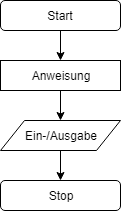
\includegraphics[height=5cm]{graph/pap_basics}
\end{figure}
\end{frame}

\begin{frame}{Elemente von Programmablaufplänen}{Verzweigungen}
\begin{figure}
    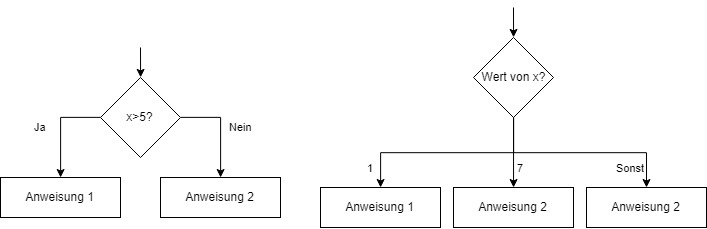
\includegraphics[width=0.9\textwidth]{graph/pap_decision}
\end{figure}
\end{frame}



\begin{frame}{Elemente von Programmablaufplänen}{Schleifen}
\begin{figure}
    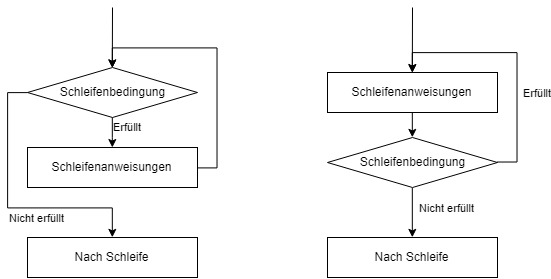
\includegraphics[height=5cm]{graph/pap_loops}
\end{figure}
\end{frame}

\begin{frame}{Elemente von Programmablaufplänen}{Zählschleifen}
\begin{figure}
    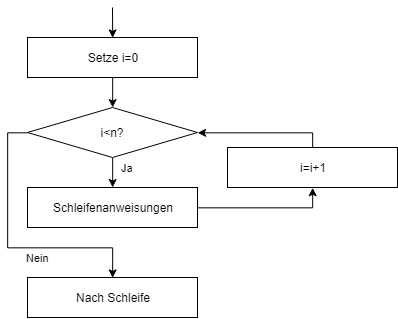
\includegraphics[height=5cm]{graph/pap_forloop}
\end{figure}
\end{frame}

\begin{frame}{Programmablaufplan}{...für unseren Algorithmus}
\begin{onlyenv}
\begin{figure}
    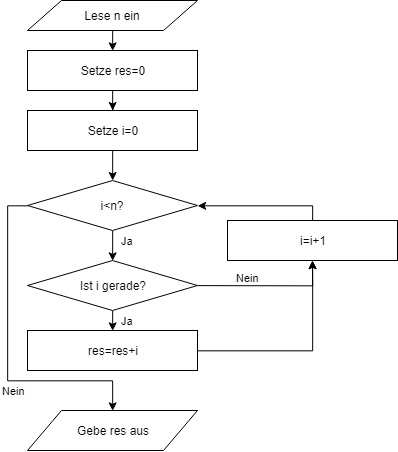
\includegraphics[height=5cm]{graph/pap_sumeven}
\end{figure}
\end{onlyenv}
\end{frame}

\begin{frame}{Zusammenfassung}
    \begin{itemize}[<+->]
        \item Keine der dargestellten Formen ist optimal
        \item Verwendung kommt auf Anforderungen und persönliche Vorlieben an
        \item Keine der hier vorgestellten Methoden zur Abbildung komplexerer objektorientierter Zusammenhänge möglich
        \item Weitere Darstellungsformen:
        \begin{itemize}
            \item Aktivitätsdiagramm
            \item Petrinetze
            \item Interaktionsdiagramme
        \end{itemize}
    \end{itemize}
\end{frame}

    \outlineFrame{Analyse}

    \outlineSubframe{Korrektheit eines Algorithmus}

\begin{frame}{Korrektheit von Algorithmen}{Allgemeines}
    \begin{itemize}[<+->]
        \item Jeder Algorithmus sollte auch in allen Fällen das korrekte Ergebnis liefern...
        \item Klingt simpel, aber eindeutiger Beweis für alle Eingaben oft schwierig
        \item Testen an ausgewählten Beispielen \textbf{nicht} ausreichend
        \begin{itemize}
            \item Jedoch verringern umfangreiche Tests natürlich das Risiko eines unentdeckten Fehler
        \end{itemize}
        \item Korrektheit lässt sich im Grunde nur durch formalen Beweis zeigen
        \begin{itemize}
            \item Diese sind häufig sehr umfangreich und komplex...
            \item ...und deshalb auch nicht Teil der Vorlesung
        \end{itemize}
    \end{itemize}
\end{frame}

\begin{frame}{Korrektheit von Algorithmen}{}
\begin{minipage}{0.4\textwidth}
            \begin{figure}
                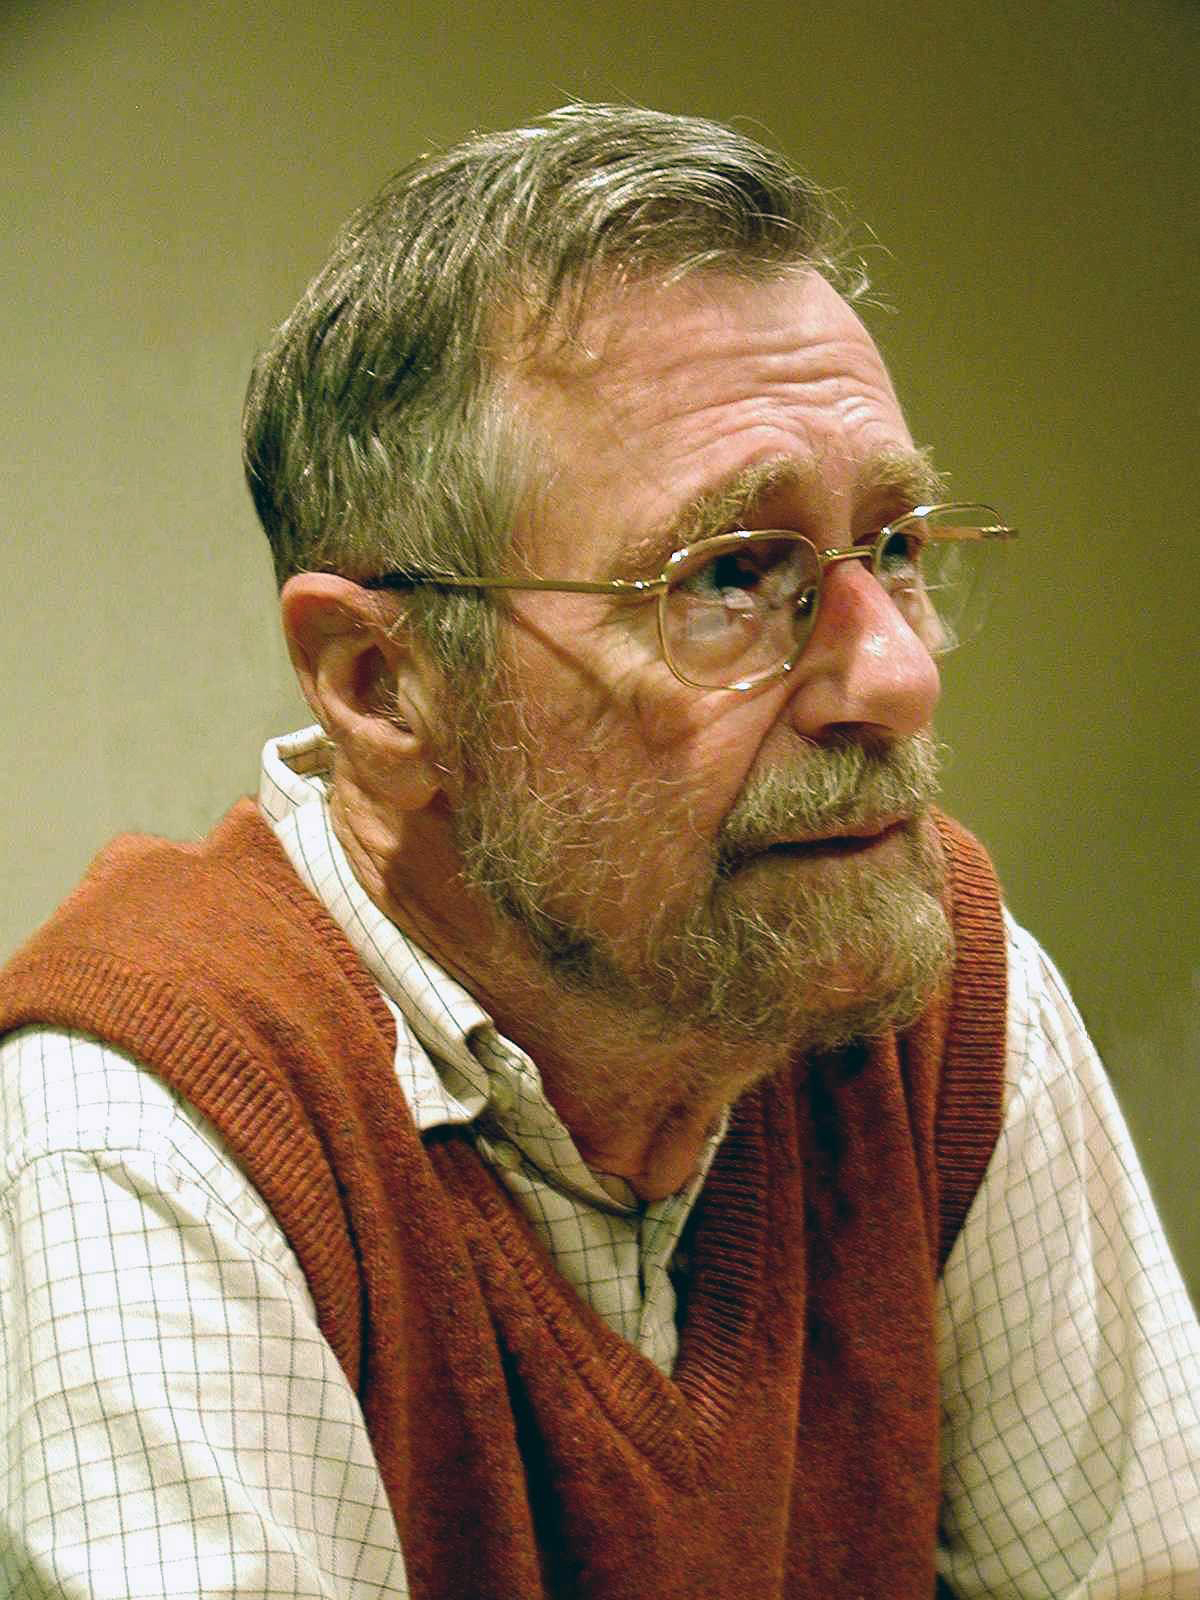
\includegraphics[height=4.5cm]{graph/dijkstra}
                \caption*{Quelle: }%\url{https://upload.wikimedia.org/wikipedia/commons/d/d9/Edsger_Wybe_Dijkstra.jpg}}
            \end{figure}
        \end{minipage}
        \hfill
        \begin{minipage}{0.55\textwidth}
            \textit{„Program testing can be used to show the presence of bugs, but never to show their absence!.“} \\\\Edsger W. Dijkstra
        \end{minipage}
\end{frame}

\outlineSubframe{Komplexitätsanalyse}

    \printbibliographyframe

	\section*{Kontakt}
	\begin{frame}{Kontakt}{}
	\begin{itemize}
		\item E-Mail: \href{mailto:lukas.abelt@airbus.com}{lukas.abelt@airbus.com}
		\item GitHub: \url{https://www.github.com/LuAbelt}
		\item GitLab: \url{https://www.gitlab.com/LuAbelt}
		\item Telefon(Firma): 07545 - 8 8895
		\item Telegram: LuAbelt
	\end{itemize}
\end{frame}
	

\end{document}